% preambolo per doppia compilazione HTML/PDF
\ifx\pdfoutput\undefined      % compilazione htlatex
\documentclass{article}
\DeclareGraphicsExtensions{.png, .gif, .jpg}
\newcommand{\href}[2]{\Link[#1]{}{} #2 \EndLink}
\newcommand{\hypertarget}[2]{\Link[]{}{#1} #2 \EndLink}
\newcommand{\hyperlink}[2]{\Link[]{#1}{} #2 \EndLink}
\else                         % compilazione pdflatex
\documentclass{article}
\usepackage{graphicx}
\usepackage{listings}
\usepackage{fancyhdr}
\usepackage{wrapfig}
\usepackage{multirow}
\usepackage{lscape}
\usepackage{amssymb,amsmath}
\pdfpagewidth 8.5in
\pdfpageheight 11in
\setlength\textwidth{5.7in}
\setlength\textheight{8.1in}
\setlength\oddsidemargin{0in}
\setlength\evensidemargin{0in}
\setlength\topmargin{-0.6in}
\setlength\footskip{0.6in}
\setlength\headsep{0.6in}
\usepackage[hyperindex]{hyperref}
\newcommand{\percent}{\,^0\!/_0}
 \hypersetup{
    bookmarks=true,         % show bookmarks bar?
    unicode=false,          % non-Latin characters in Acrobat’s bookmarks
    pdftoolbar=true,        % show Acrobat’s toolbar?
    pdfmenubar=true,        % show Acrobat’s menu?
    pdffitwindow=true,      % page fit to window when opened
    pdfauthor={Maurizio},   % author
    pdfsubject={Ungaro},    % subject of the document
    pdfnewwindow=true,      % links in new window
    colorlinks=true,        % false: boxed links; true: colored links
    linkcolor=black,        % color of internal links
    citecolor=blue,         % color of links to bibliography
    filecolor=magenta,      % color of file links
    urlcolor=blue           % color of external links
}
\fi


\begin{document}
\pagestyle{fancy}
\renewcommand{\sectionmark}[1]{\markright{\slshape \thesection\ #1}{}}
\fancyhead[R]{\bf\rightmark} 
\fancyhead[L]{e1-6 analysis}
\fancyfoot[R]{ \sl M. Ungaro, K. Joo}
\fancyfoot[L]{ \sl UCONN/JLAB}

\title{\large e1-6 $\pi^0$ selection}
 \author{M. Ungaro, K. Joo}
\maketitle

\abstract{This document describes the selection of $\pi^0$ events. 
Kinematics is used to separate Bethe-Heitler events from the
$\pi^0$ signal. The missing mass resolution gets worse as W increases, but it doesn't affect
the $\pi^0$/B.H. separation.}

\tableofcontents

\section{Bethe Heitler processes}
\label{sec:bethe}

Fig. \ref{fig:wmm_after_fiducial}  shows the $(e,P)$ missing mass $M_X^2$ versus $W$
distribution for the e1-6 period after electron and proton ID, vertex correction
and selection, fiducial cuts and kinematic corrections.
The elastic and Bethe Heitler (B.H.) events, illustrated in Fig. \ref{fig:bethe},	are
 seen at $M_X^2=0$, with the characteristic increase of the cross section
at high $W$. Also shown are the $S_{11}(1535)$ resonance decaying in $(P, \eta)$,
the $P_{13}(1720)$ resonance decaying in $(P, \rho)$ and the subject of this analysis, the
$\Delta^{+}(1232)$ resonance decaying in $(P, \pi^0)$.

\begin{figure}[ht]
\centering
	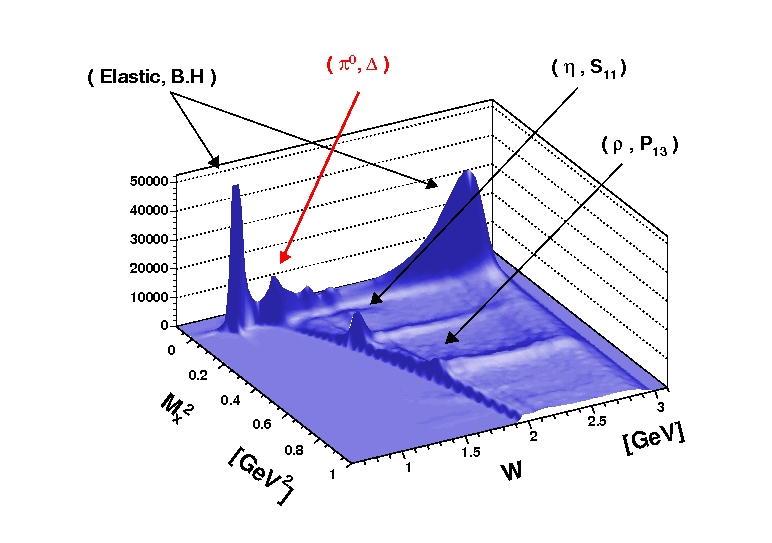
\includegraphics[width=0.98\textwidth ]{img/wmm_after_fiducial.jpg}
	\caption{$(e,P)$ Missing mass $M_X^2$ versus $W$after electron and proton ID, vertex correction
	and selection, fiducial cuts and kinematic corrections for the e1-6 data.
	The elastic and B.H. events are visible at $M_X^2=0$. Also visible are the $S_{11}\rightarrow (P, \eta)$,
	the $P_{13}\rightarrow (P, \rho)$ and of course the $\Delta^{+}\rightarrow (P, \pi^0)$ events. }
		\label{fig:wmm_after_fiducial}
\end{figure}

\vspace{1cm}

The missing mass technique alone cannot separate the B.H. processes from the
$\pi^0$ events efficiently because of the limited resolution, especially at high W.
What follows is the documentation of the kinematic cuts used to remove the B.H. events from
the inelastic data.

\clearpage\newpage

The typical angle between the emitted photon and the electron in B.H. processes is $\theta \sim m_e/E_e$
where $m_e$ is the electron mass and $E_e$ its energy \cite{bib:motsai}, \cite{bib:andrei_private}.
Even at the lowest electron energies detected in CLAS, this
corresponds to fractions of milliradians and can be used to select B.H. events effectively, since the electron
does not change its direction when emitting the photon. As a consequence, B.H. processes are mostly coplanar.

Due to resolution effects, this coplanarity is best seen in different variables at different W. We describe the
use of these different variables in the next sections.



\vspace{0.7 cm}
\begin{figure}[ht]
	\centering
		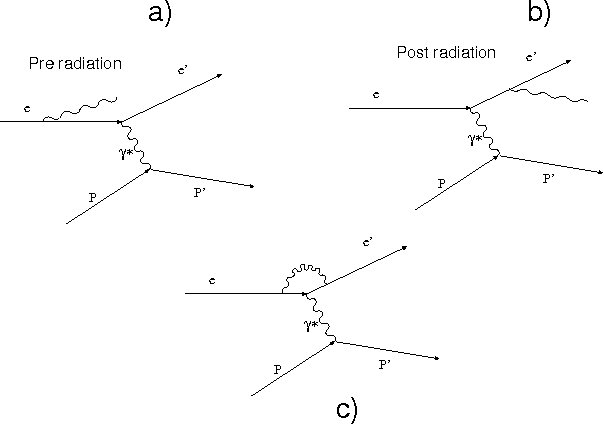
\includegraphics[width=0.72\textwidth ]{img/bethe.jpg}
		\caption{Bethe Heitler events contributing to the (eP) final state leaking into
		the $\pi^0$ missing mass. }
			\label{fig:bethe}
\end{figure}



\subsection{Coplanarity Cut}
The angle $\Delta\phi = \phi_e-\phi_P$ is plotted in Fig. \ref{fig:dphi_epXmm2_no_cut} as a function
of $M_X^2$ for different W bins. One can see the B.H. events at $\Delta\phi \sim 180^0$ and $M_X^2 = 0$.
As W increases, the $M_X^2$ resolution worsen, but the B.H. events stay localized at $\Delta\phi \sim 180^0$.
The $\Delta\phi$ distributions are fitted with a gaussian plus second order polynomial as shown in Fig. \ref{fig:dphi_no_cut}.
The mean and sigma of those fit are summarized in Fig. \ref{fig:dphi_fits}. Both mean and sigma
are independent of W. Events within 4 sigma of the mean are rejected.

\begin{landscape}
	\begin{figure}[ht]
	\centering
		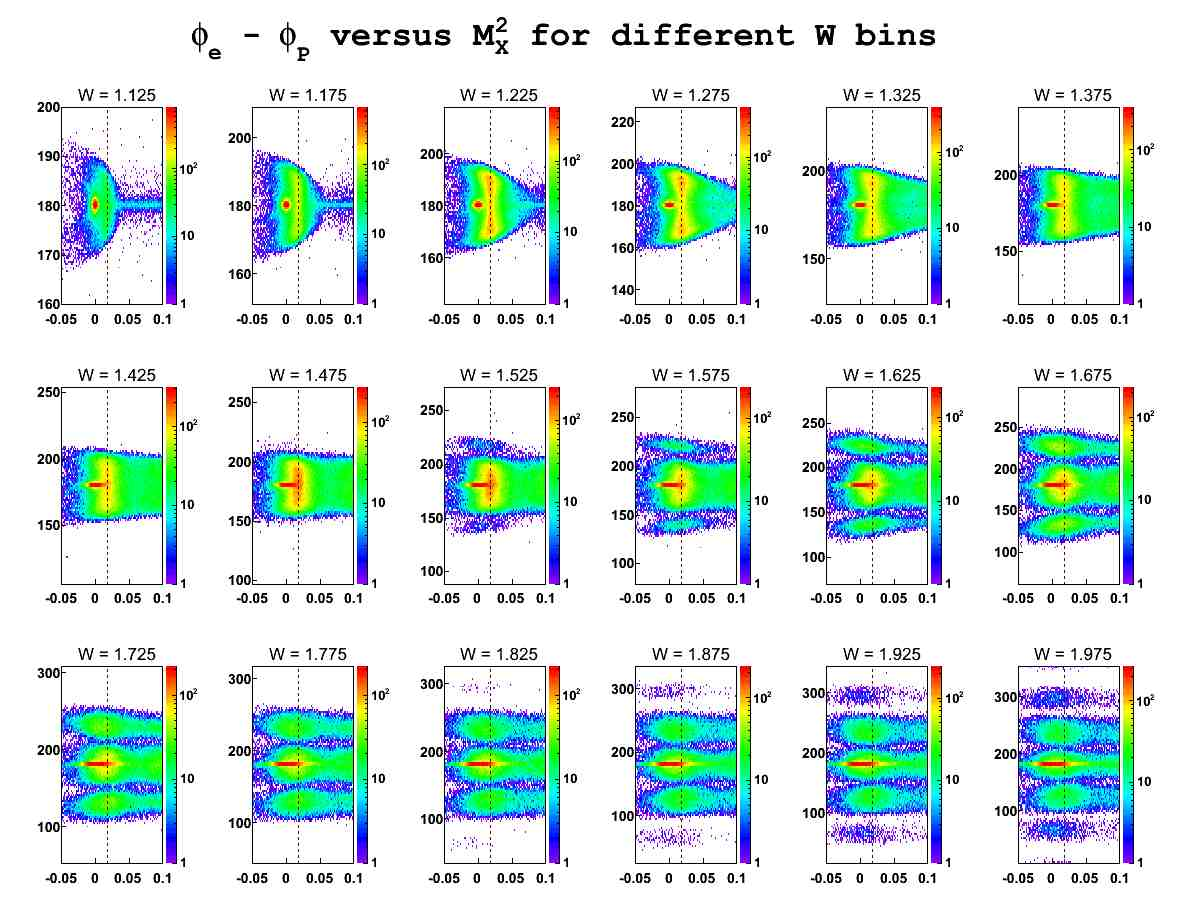
\includegraphics[width=1.15\textheight]{img/dphi_epXmm2_no_cut.jpg}
		\caption{$\Delta\phi = \phi_e-\phi_P$ versos $M_X^2$ for different W. The B.H. events
		are visible at $\Delta\phi \sim 180^0$ and $M_X^2 = 0$. The vertical dotted line is at the
		$\pi^0$ mass. As W increases, the $M_X^2$ resolution worsen, but the B.H. events
		stay localized at $\Delta\phi \sim 180^0$.}
		\label{fig:dphi_epXmm2_no_cut}
	\end{figure}
\end{landscape}
\clearpage\newpage

\begin{landscape}
	\begin{figure}[ht]
	\centering
		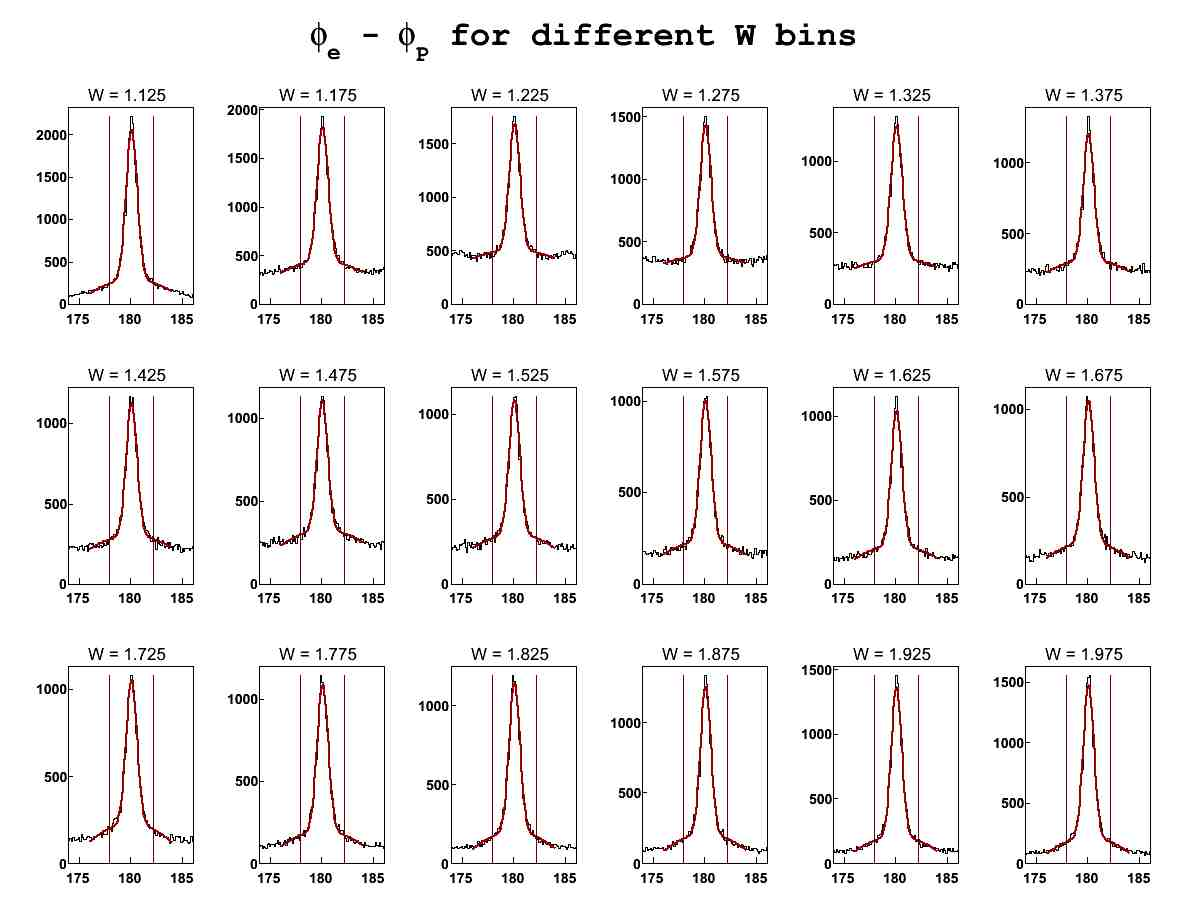
\includegraphics[width=1.15\textheight]{img/dphi_no_cut.jpg}
		\caption{Fits to the $\Delta\phi$ distributions for different W bins. The function used was
		a gaussian plus second order polynomial.}
		\label{fig:dphi_no_cut}
	\end{figure}
\end{landscape}

\begin{figure}[ht]
	\centering
	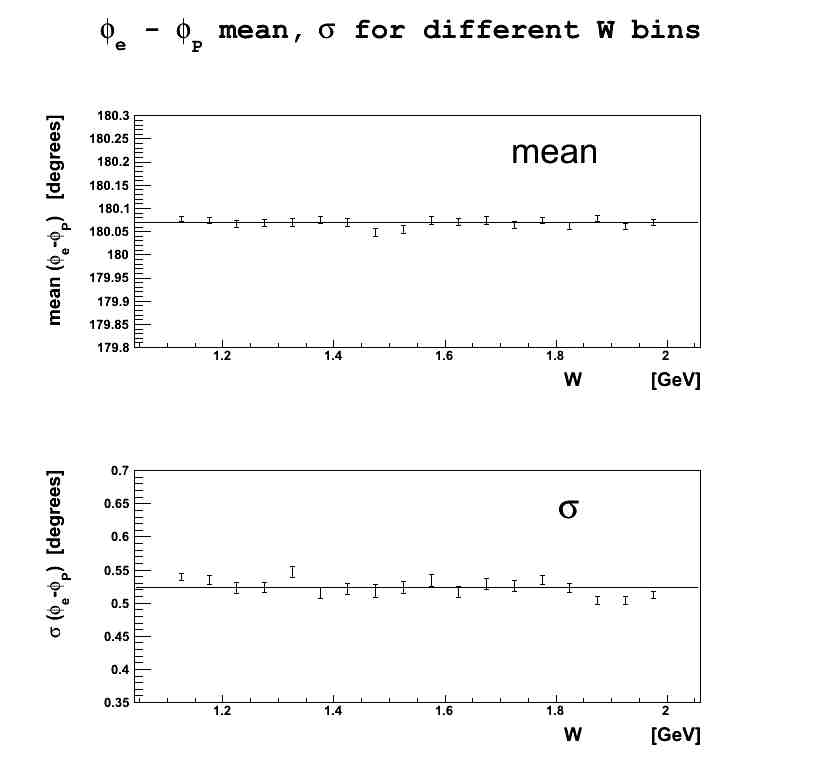
\includegraphics[width=0.95\textwidth]{img/dphi_fits.jpg}
	\caption{Mean and sigma of the $\Delta\phi$ fits as a function of W. Both mean and sigma
	are independent of W. Events within 4 sigma of the mean are rejected. }
		\label{fig:dphi_fits}
\end{figure}
\clearpage\newpage

\subsection{Post-radiative events Cut}
Using elastic kinematics, one can calculate the proton angle in the lab $\theta^P_{calc}$
using only the scattered electron angle $\theta_{e'}$ and the beam energy $E$:
$$
\tan\theta^P_{calc} =  \frac{1}{(1+\frac{E}{M_P})\tan\frac{\theta_{e'}}{2}}
$$
This calculation is independent of the outgoing electron energy and therefore is valid for
all post-radiative effects shown in Fig. \ref{fig:bethe} b).
Thus the difference between $\theta^P_{calc}$ and the measured proton angle
$\Delta\theta_{post} = \theta^P_{calc} - \theta^P_{meas} $ is 0 for post-radiation.


$\Delta\theta_{post}$ is plotted in Fig. \ref{fig:dth1_epXmm2_no_cut}
for different W bins. The post-radiative tail can be seen at $\Delta\theta_{post}=0$.
Its strength diminish as W increases but its non null at all W.
The $\Delta\theta_{post}$ distributions are fitted with a gaussian plus second order polynomial
as shown in Fig. \ref{fig:dth1_no_cut}. The mean and sigma of those fit are summarized in Fig. \ref{fig:dth1_fits}.
Both mean and sigma are independent of W. Events within 4 sigma if the mean are rejected.

\subsection{Pre-radiative events Cut}
Using elastic kinematics, one can calculate the proton angle in the lab $\theta^P_{calc}$
using only the scattered electron energy $E'$ and angle $\theta_{e'}$:

$$
\tan\theta^P_{calc2} =  \frac{1}{(1+\frac{E'}{M_P-E'+E'\cos\theta_{e'}})\tan\frac{\theta_{e'}}{2}}
$$

This calculation is independent of the incident electron energy and therefore is valid for
all pre-radiative effects shown in Fig. \ref{fig:bethe} a).
Thus the difference between $\theta^P_{calc2}$ and the measured proton angle
$\Delta\theta_{pre} = \theta^P_{calc2} - \theta^P_{meas}$ is 0 for pre-radiation.


$\Delta\theta_{pre}$ is plotted in Fig. \ref{fig:dth2_epXmm2_no_cut}
for different W bins. The pre-radiative tail can be seen at $\Delta\theta_{pre}=0$.
Its strength increases with W.
The $\Delta\theta_{pre}$ distributions are fitted with a gaussian plus second order polynomial
as shown in Fig. \ref{fig:dth2_no_cut}. The mean and sigma of those fit are summarized in Fig. \ref{fig:dth2_fits}.
The mean decreases slightly with W. The sigma is independent of W. Events with
$\Delta\theta_{pre} < mean + 4\sigma$ are rejected.	
	

\begin{landscape}
	\begin{figure}[ht]
	\centering
		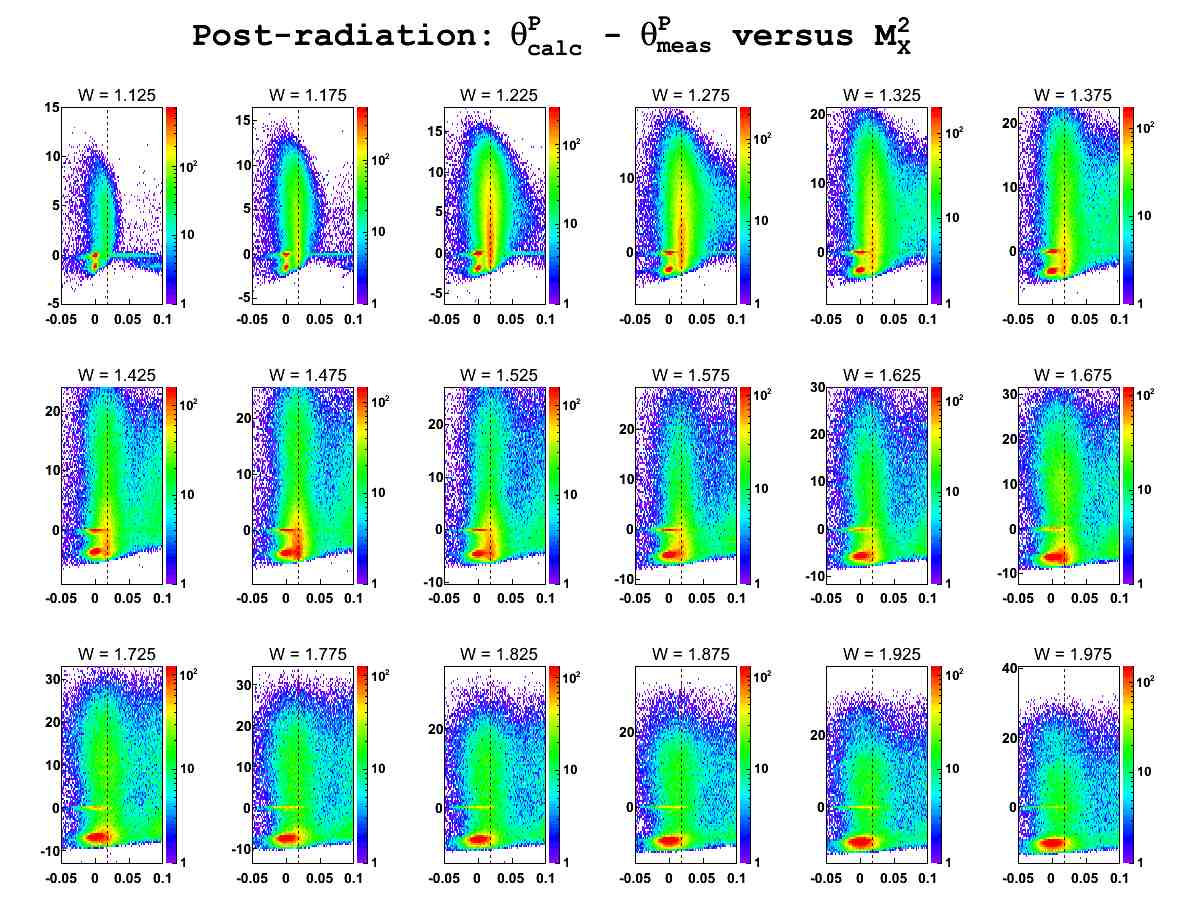
\includegraphics[width=1.15\textheight]{img/dth1_epXmm2_no_cut.jpg}
		\caption{$\Delta\theta_{post}$ is zero for post-radiative tail. The number of post-radiative
		        events diminish as W increases.}
		\label{fig:dth1_epXmm2_no_cut}
	\end{figure}
\end{landscape}
\clearpage\newpage

\begin{landscape}
	\begin{figure}[ht]
	\centering
		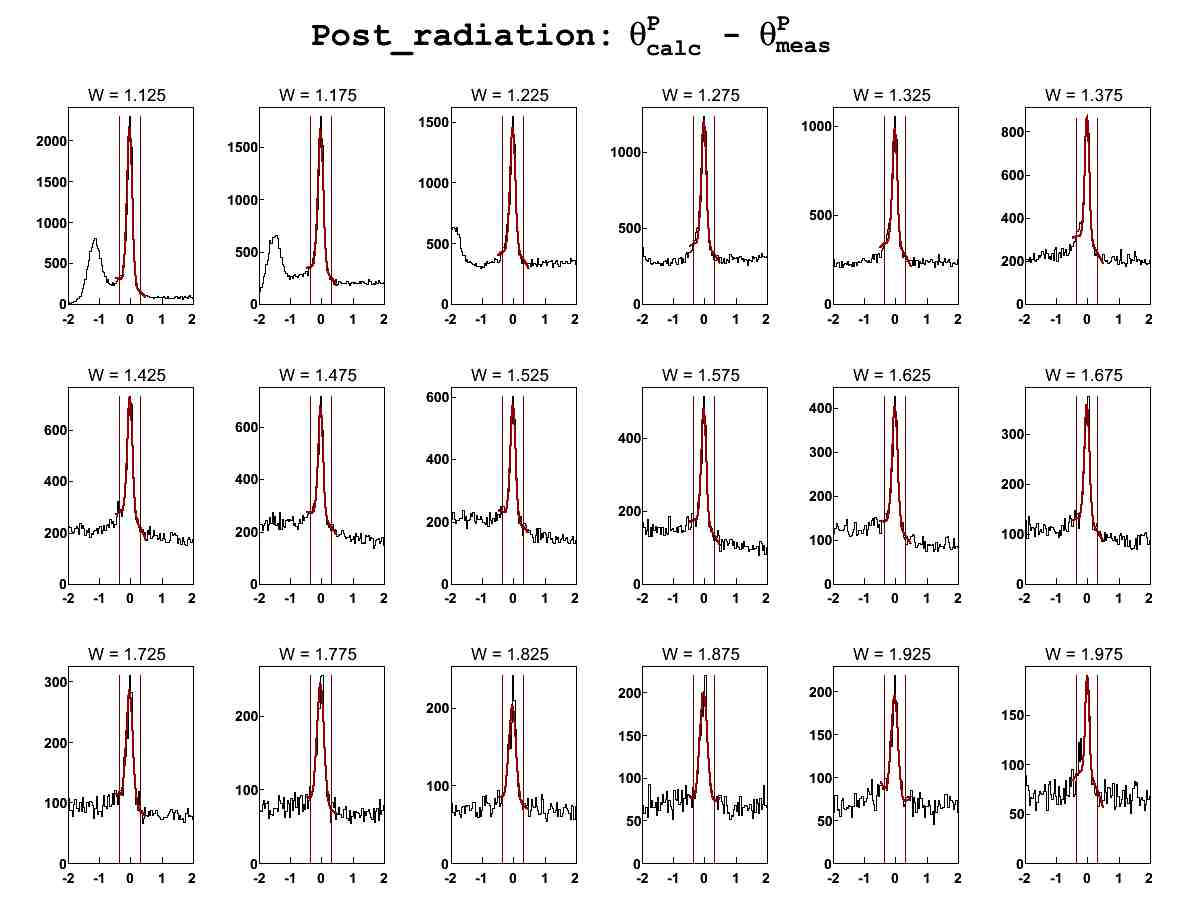
\includegraphics[width=1.15\textheight]{img/dth1_no_cut.jpg}
		\caption{Fits to the $\Delta\theta_{post}$ distributions. The function used is a gaussian plus
		second order polynomial.}
		\label{fig:dth1_no_cut}
	\end{figure}
\end{landscape}

\begin{figure}[ht]
	\centering
	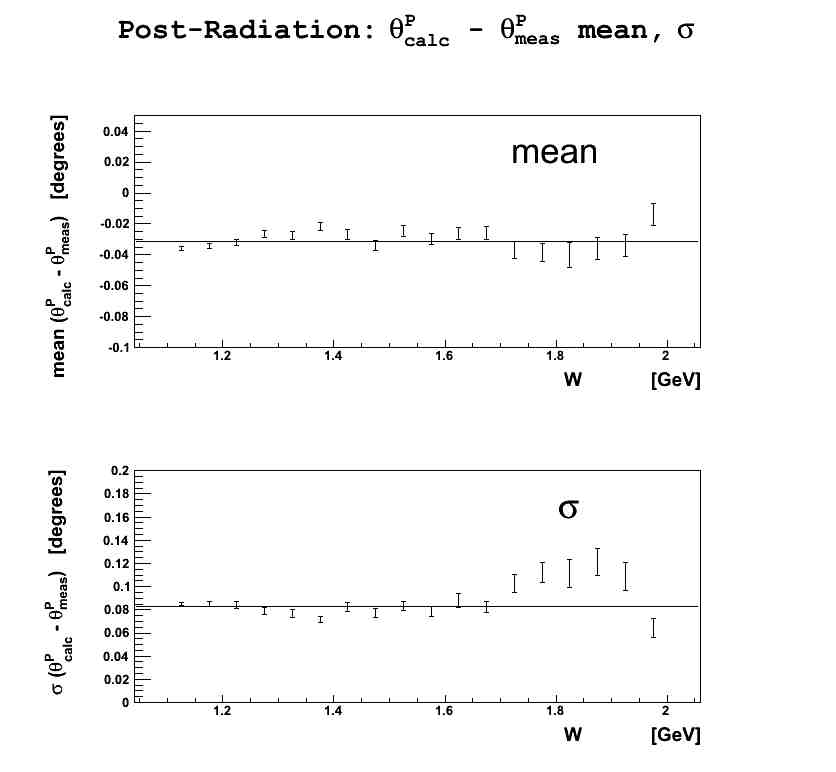
\includegraphics[width=0.95\textwidth]{img/dth1_fits.jpg}
	\caption{The mean and sigma of the $\Delta\theta_{post}$ distributions. Both mean and sigma are
	independent of W. Events within 4 sigma if the mean are rejected.}
	\label{fig:dth1_fits}
\end{figure}
\clearpage\newpage



\begin{landscape}
	\begin{figure}[ht]
	\centering
		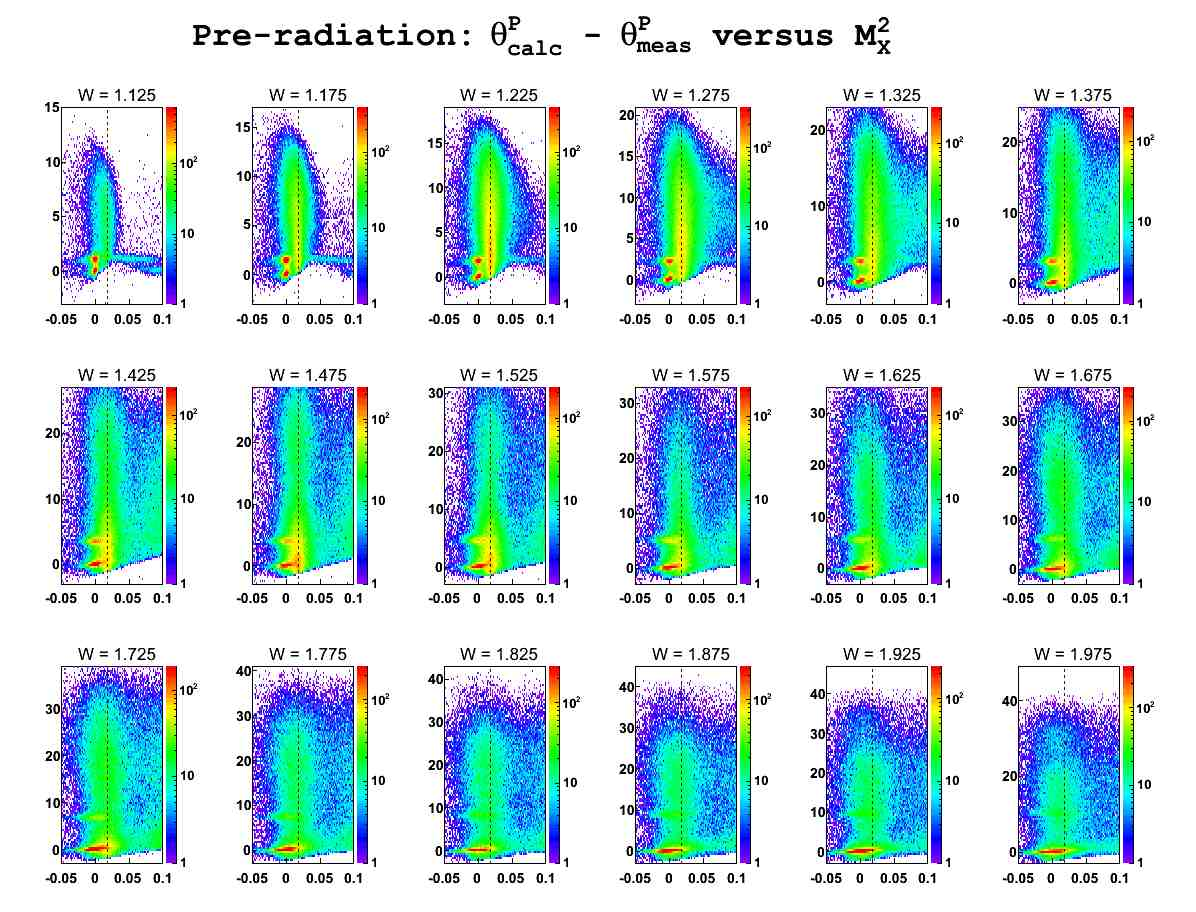
\includegraphics[width=1.15\textheight]{img/dth2_epXmm2_no_cut.jpg}
		\caption{$\Delta\theta_{pre}$ is zero for pre-radiative tail. The number of post-radiative
		events increases as W increases.}
	\label{fig:dth2_epXmm2_no_cut}
	\end{figure}
\end{landscape}
\clearpage\newpage

\begin{landscape}
	\begin{figure}[ht]
	\centering
		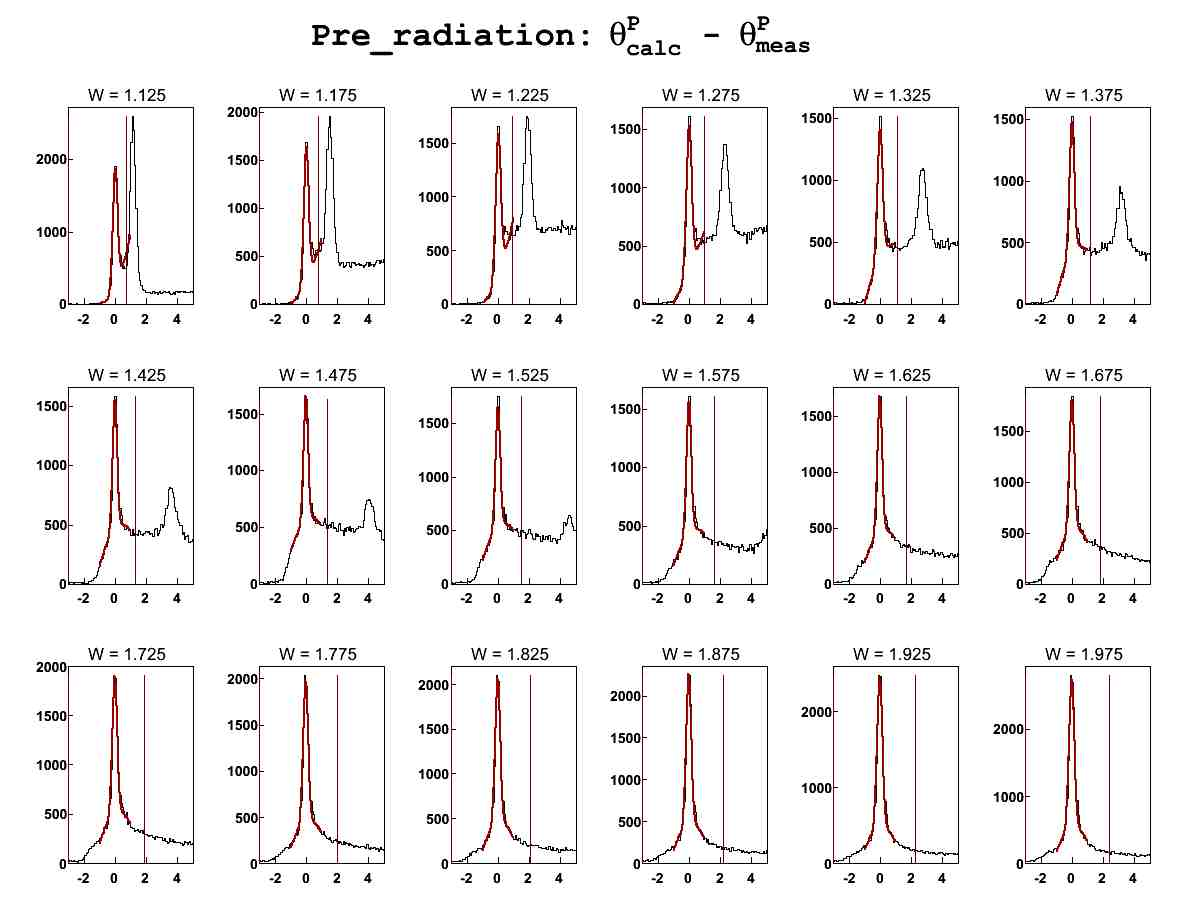
\includegraphics[width=1.15\textheight]{img/dth2_no_cut.jpg}
		\caption{Fits to the $\Delta\theta_{pre}$ distributions. The function used is a gaussian plus
		second order polynomial.}
		\label{fig:dth2_no_cut}
	\end{figure}
\end{landscape}

\begin{figure}[ht]
	\centering
		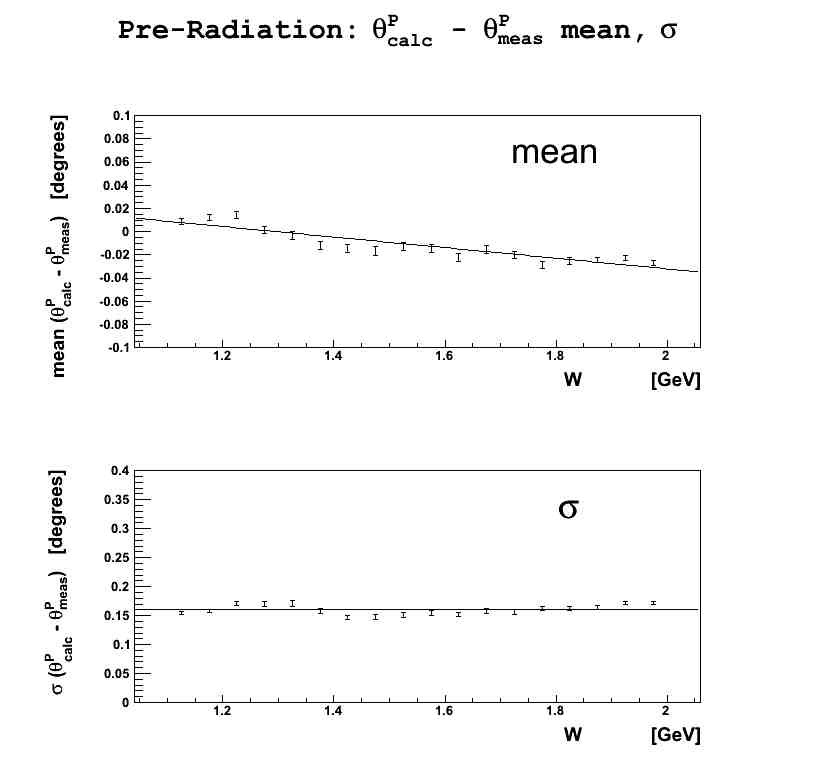
\includegraphics[width=0.95\textwidth]{img/dth2_fits.jpg}
		\caption{The mean and sigma of the $\Delta\theta_{pre}$ distributions. The mean decreases
		slightly with W. The sigma independent of W. Events with $\Delta\theta_{pre} < mean + 4\sigma$
		are rejected.}
	\label{fig:dth2_fits}
\end{figure}

\clearpage\newpage
\section{Results}
The W and $M_X^2$,  before (black) and after (red) distributions are shown in Fig. \ref{fig:wmm_pi0}.
The W vs $M_X^2$ distribution for the filtered events is shown in   Fig. \ref{fig:w_mm_pi0} . The $\Delta\phi$, $\Delta\theta_{post}$ 
and $\Delta\theta_{pre}$ distributons for the filtered events are shown in 

\begin{figure}[ht]
	\centering
		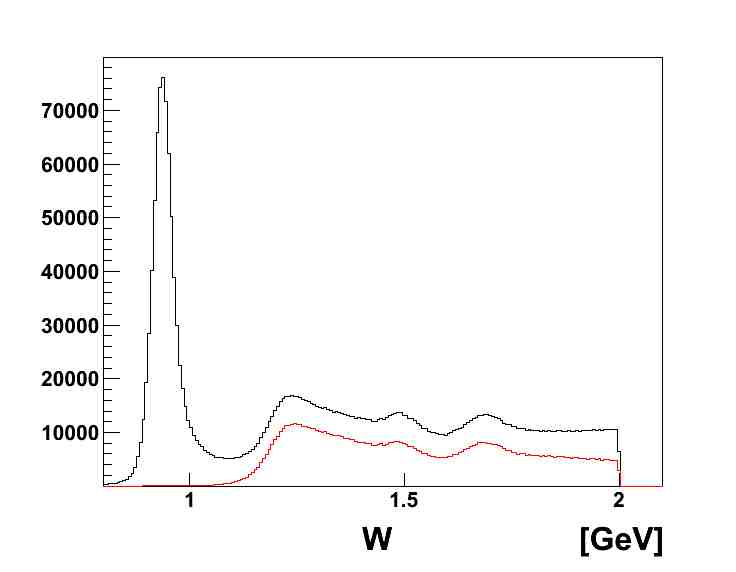
\includegraphics[width=0.65\textwidth]{img/W.jpg}
		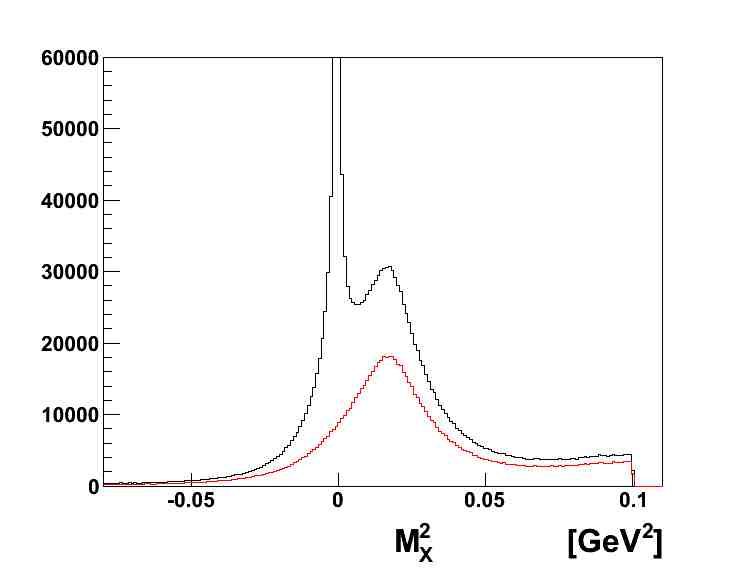
\includegraphics[width=0.65\textwidth]{img/mm.jpg}
		\caption{W (top) and missing mass (bottom) distributions for all (black) and filtered (red) events. 
		No cuts on W or missing mass are applied. }
	\label{fig:wmm_pi0}
\end{figure}



\begin{figure}[hb]
	\centering
		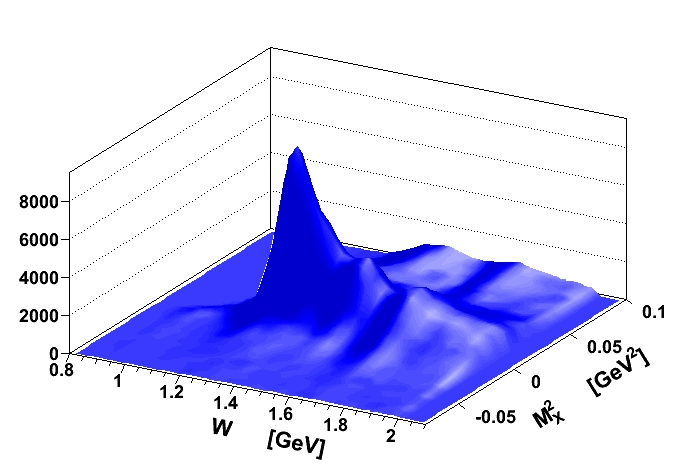
\includegraphics[width=0.9\textwidth]{img/w_mm.jpg}
		\caption{W vs $M_X^2$ distribution for the filtered events.  }
	\label{fig:w_mm_pi0}
\end{figure}
\clearpage\newpage

\begin{landscape}
	\begin{figure}[ht]
	\centering
		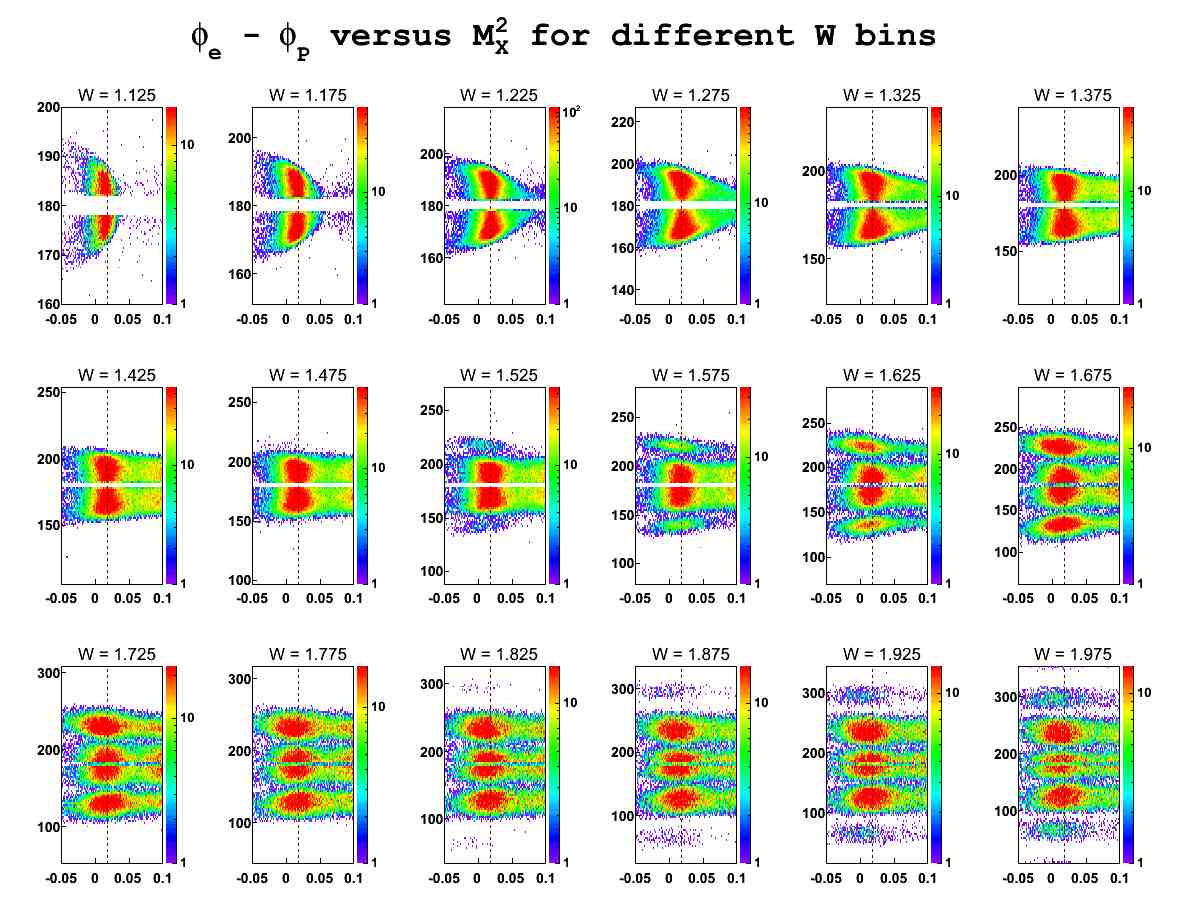
\includegraphics[width=1.15\textheight]{img/dphi_epXmm2_all_cuts.jpg}
		\caption{$\Delta\phi$ versus missing mass for the filtered events.}
	\label{fig:dphi_epXmm2_all_cuts}
	\end{figure}
\end{landscape}


\begin{landscape}
	\begin{figure}[ht]
	\centering
		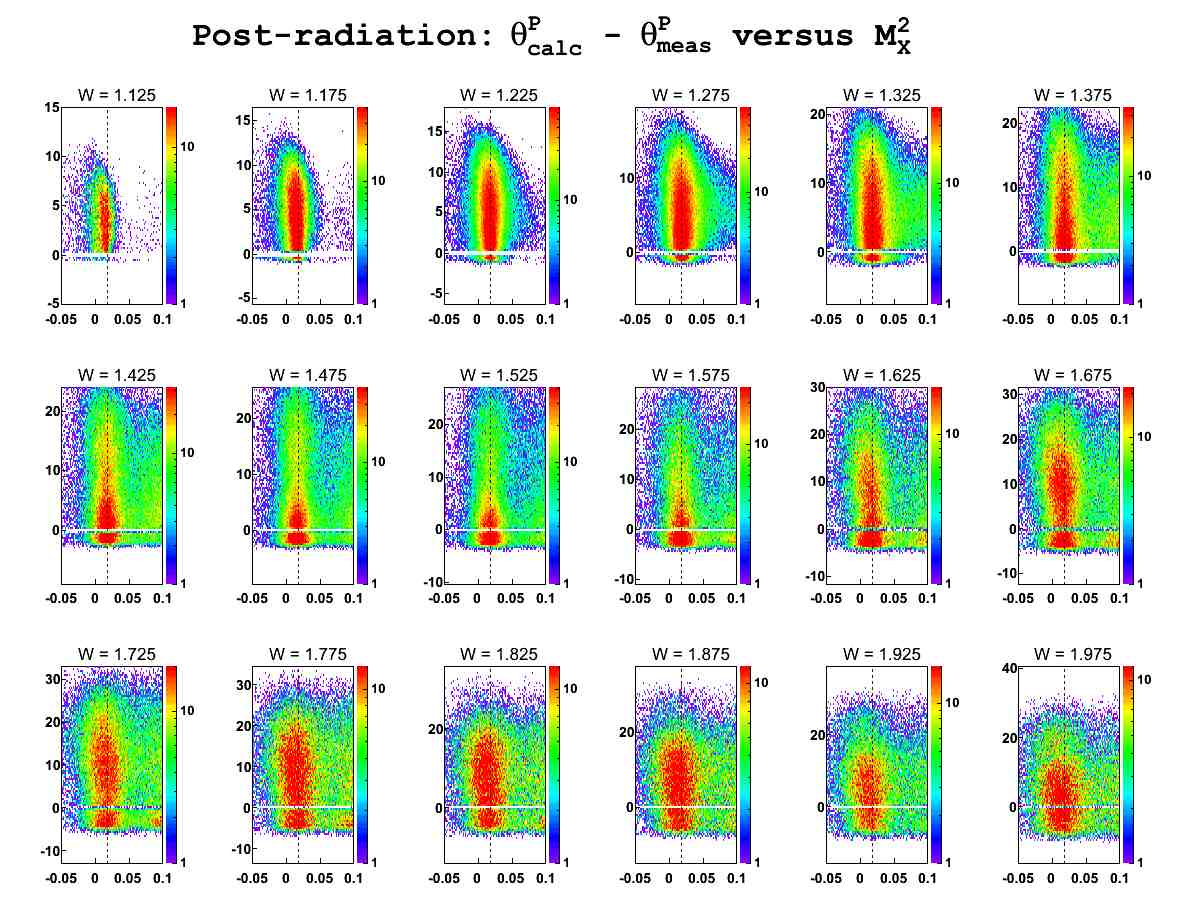
\includegraphics[width=1.15\textheight]{img/dth1_epXmm2_all_cuts.jpg}
		\caption{$\Delta\theta_{post}$ versus missing mass for the filtered events.}
	\label{fig:dth1_epXmm2_all_cuts}
	\end{figure}
\end{landscape}


\begin{landscape}
	\begin{figure}[ht]
	\centering
		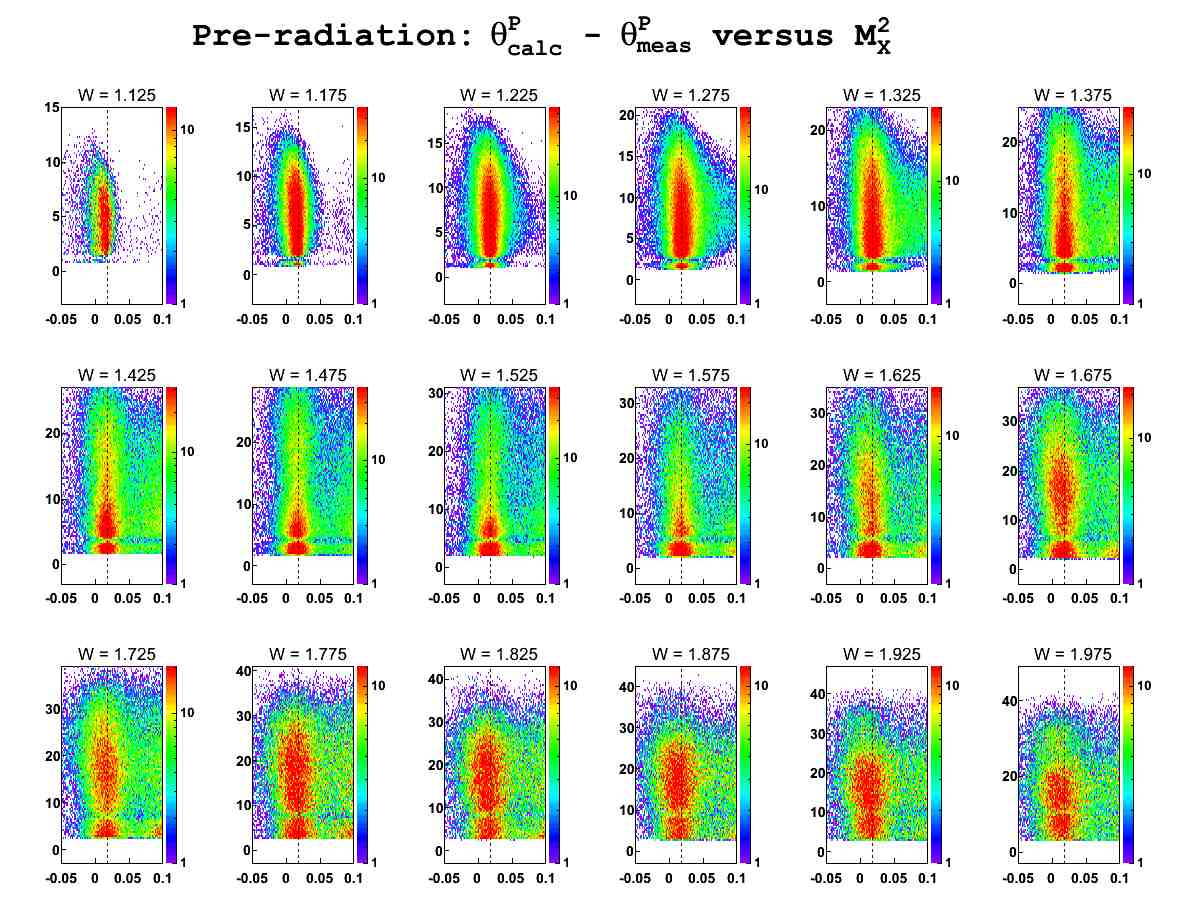
\includegraphics[width=1.15\textheight]{img/dth2_epXmm2_all_cuts.jpg}
		\caption{$\Delta\theta_{pre}$ versus missing mass for the filtered events.}
	\label{fig:dth2_epXmm2_all_cuts}
	\end{figure}
\end{landscape}




\clearpage\newpage

\section{Bethe Heitler Simulation}
To check the effectiveness of these cuts, elastic events were simulated with radiative tail.
The Bethe Heitler calculation is made by modifying the elastic peak by vertex corrections
according to the Mo-Tsai formula (II.6) and internal bremmstrahlung (radiative tails) calculated from
a Monte-Carlo sampling of formula (B.4) from RMP, Vol. 41, 205 (1969) \cite{bib:elast_gen}.

The 

\begin{landscape}
\begin{figure}[ht]
\centering
\includegraphics[width=1.15\textheight]{img/epXmm2_W_data_no_cut.gif}
\caption{$\Delta\theta_{pre}$ versus missing mass for the filtered events.}
\label{fig:dth2_epXmm2_all_cuts}
\end{figure}
\end{landscape}













\begin{thebibliography}{mybib}
 \bibitem {bib:motsai}            {Mo and Tsai},                              \textit{Rev. Mod. Phys. {\bf 41} (1969)}
 \bibitem {bib:andrei_private}    {Andrei Afanaciev},                          \textit{Private Communication}
 \bibitem {bib:elast_gen}         {R. Minehart, K. Joo and L.C. Smith},        \href{http://clasweb.jlab.org/cgi-bin/cvsweb/cvsweb.cgi/packages/aao/elast_gen}{elast\_gen software}
\end{thebibliography}


\end{document}








